\documentclass[12pt]{report}
\usepackage[utf8]{inputenc} 
\usepackage[russian]{babel} 
\usepackage{amsmath} 
\usepackage{hyperref} 
\usepackage{graphicx}
\usepackage{amssymb}
\usepackage{wrapfig}
\usepackage{bbm}
\usepackage{parskip}
\usepackage{gensymb}
\usepackage{multicol}
\usepackage{array}
\usepackage{stackengine}
\usepackage{mathtools}
\usepackage[final]{pdfpages}
\parindent 0pt
\parskip 6pt
\newcommand{\numberset}[1]{\mathbb{#1}} 
\newcommand{\Aop}{\mathcal{A}}
\newcommand{\Bop}{\mathcal{B}}
\newcommand{\N}{\numberset{N}}
\newcommand{\Q}{\mathbb{Q}}
\newcommand{\R}{\mathbb{R}}
\newcommand{\Z}{\mathbb{Z}}
\newcommand{\Eps}{\mathcal{E}}
\newcommand{\Zero}{\mathbb{O}}
\newcommand{\Compl}{\mathbb{C}}
\newcommand{\n}{\bigbreak}
\usepackage[a4paper, total={6in, 8in}]{geometry}
\usepackage{color}
\usepackage{hyperref}
\def\letus{%
    \mathord{\setbox0=\hbox{$\exists$}%
             \hbox{\kern 0.125\wd0%
                   \vbox to \ht0{%
                      \hrule width 0.75\wd0%
                      \vfill%
                      \hrule width 0.75\wd0}%
                   \vrule height \ht0%
                   \kern 0.125\wd0}%
           }%
}
\DeclarePairedDelimiter\evaluat{.}{\rvert}
\reDeclarePairedDelimiterInnerWrapper\evaluat{nostar}{\mathopen{}#2\mathclose{#3}}
\hypersetup{
    colorlinks=true,
    linkcolor=blue,
    urlcolor=blue,
    linktoc=all
}
\begin{document}
\begin{titlepage}
	\centering
	{\scshape\LARGE Группа M3235\protect\\Команда №4 \par}
	\vspace{1cm}
	{\scshape\Large Математический анализ\par}
	\vspace{1.5cm}
	{\huge\bfseries Типовой расчёт №1\par}
	\vspace{2cm}
	{\Large\itshape Олеся Чеботарёва\protect\\Ирина Ткаченко\protect\\Андрей Сухарев\protect\\Николай Тананыкин \par}
	\vfill
	\vfill
	{\large Октябрь 2019, 3 семестр \par}
\end{titlepage}
\tableofcontents
\newpage
\chapter{Дифференцируемость функции двух переменных в точке}
Дана функция
$$ f(x,y)=\sin\Big(\frac{\pi}{4}+\sqrt[3]{xy^2}\Big) $$
Выяснить, является ли заданная функция дифференцируемой в точке $M(0, 0)$. Построить график этой функции (поверхность). 

Построить плоскость $z-z_0=x\cfrac{\partial f}{\partial x}(0,0)+y\cfrac{\partial f}{\partial y}(0,0)$. Является ли эта плоскость касательной к поверхности?
\newpage
\paragraph{График функции (\href{https://www.geogebra.org/3d/kjp5s8yt}{нажми на меня})}
\begin{center}
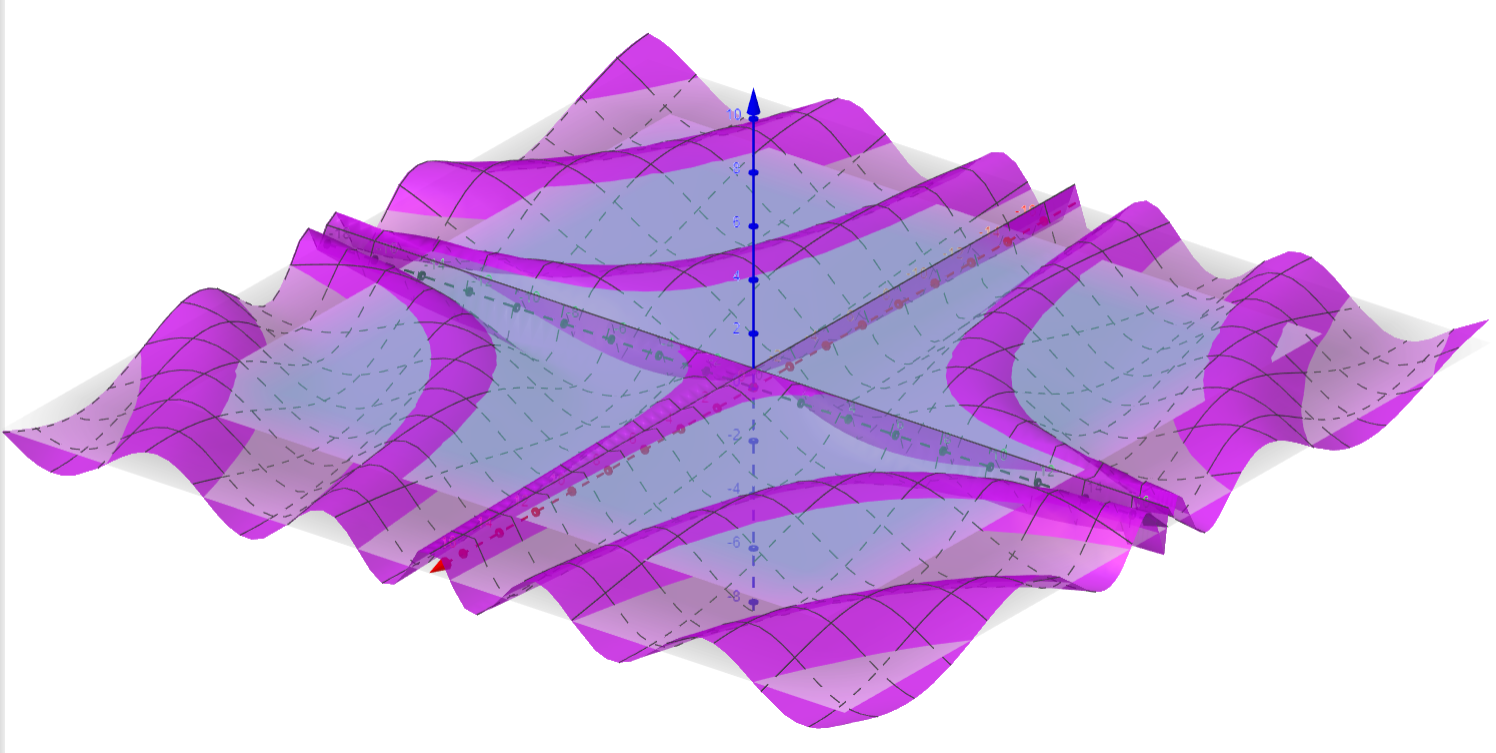
\includegraphics[scale=0.45]{task1.png}
\end{center}
Функция является дифференцируемой, если $f(x,y)=f(x_0,y_0)+\cfrac{\partial f}{\partial x}\Delta x+\cfrac{\partial f}{\partial y}\Delta y+o(r)$, где $r=\|\Delta x,\,\Delta y\|=\sqrt{(\Delta x)^2+(\Delta y)^2}$ и $\Delta x=x-x_0,\,\Delta y=y-y_0$. Найдём производные в окрестности точки $M$:
$$ \cfrac{\partial f}{\partial x}(0,0) = \lim_{(x,y)\to 0}\cfrac{\sin\Big(\frac{\pi}{4}+\sqrt[3]{(x-\Delta x)y^2}\Big)-\sin\Big(\frac{\pi}{4}+\sqrt[3]{xy^2}\Big)}{\Delta x}=0,\quad \cfrac{\partial f}{\partial y}(0,0) =0 $$
При вычисленных выше значениях проверим равенство $\sin\Big(\frac{\pi}{4}+\sqrt[3]{xy^2}\Big)-\frac{1}{\sqrt{2}}=o(\sqrt{x^2-y^2})$.

Теория: $m$ является $o$ малым от $n$, если $\lim \frac{|m|}{|n|}=0$. Тогда:
$$ \lim_{(x,y)\to(0,0)}\left|\cfrac{\sin\Bigg(\cfrac{\pi}{4}+\sqrt[3]{xy^2}\Bigg)-\cfrac{1}{\sqrt{2}}}{\sqrt{x^2+y^2}}\right|=\lim_{(x,y)\to(0,0)}\cfrac{\left|2\sin\sqrt[3]{xy^2}\cdot\cos\Bigg(\cfrac{\pi}{4}+\cfrac{\sqrt[3]{xy^2}}{2}\Bigg)\right|}{\sqrt{x^2+y^2}}=$$

$$=\lim_{(x,y)\to(0,0)}\cfrac{\sqrt[3]{xy^2}}{\sqrt{x^2+y^2}}=\cfrac{|\sqrt[3]{r^3\cos\varphi\cdot\sin^2\varphi}|}{r}=\left|\sqrt[3]{\cos\cfrac{\pi}{3}\sin^2\cfrac{\pi}{3}}\right|  $$
$\letus\,\varphi=\cfrac{\pi}{3}$, тогда:
$$ \lim_{(x,y)\to(0,0)}\cfrac{\left|\sin\Bigg(\cfrac{\pi}{4}+\sqrt[3]{xy^2}\Bigg)-\cfrac{1}{\sqrt{2}}\right|}{\sqrt{x^2+y^2}}=\left|\sqrt[3]{\cos\cfrac{\pi}{3}\sin^2\cfrac{\pi}{3}}\right|\neq 0 $$
Следовательно, $\sin\Big(\frac{\pi}{4}+\sqrt[3]{xy^2}\Big)-\frac{1}{\sqrt{2}}\ne o(\sqrt{x^2-y^2})$. Следовательно, \textbf{функция не дифференцируема}.

Плоскость $z-z_0=x\cfrac{\partial f}{\partial x}(0,0)+y\cfrac{\partial f}{\partial y}(0,0)=0$ является плоскостью $z=\cfrac{1}{\sqrt{2}}$. На графике выше она изображена голубым цветом. Она является касательной к нашей поверхности по определнию:

\begin{center}
    \fbox{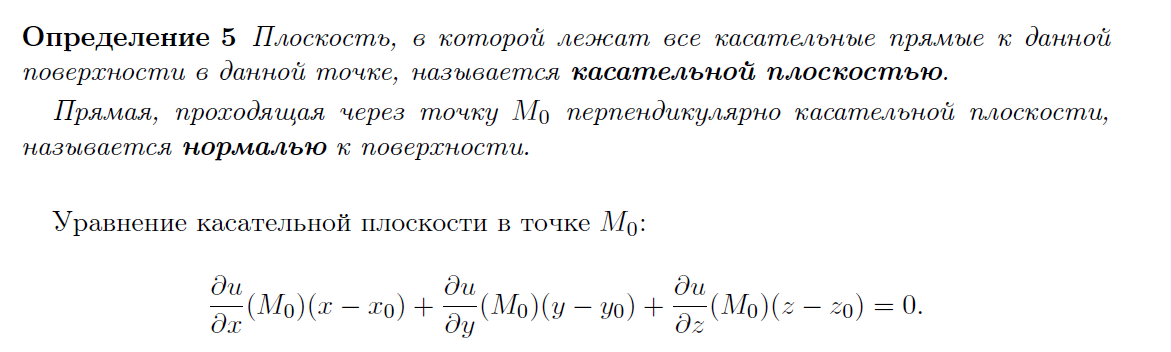
\includegraphics[scale=0.65]{task_1.png}}
\end{center}

P.S.: красным цветом изображена ось $Ox$, зелёным цветом ось $Oy$, синим цветом ось $Oz$.
\chapter{Наибольшее и наименьшее значение функции двух
переменных в области}
Даны три точки: $A(0,0,12)$, $B(0,0,4)$ и $C(8,0,8)$. На плоскости $Oxy$ найдите такую точку $D$, чтобы сфера, проходящая через $A$, $B$, $C$ и $D$, имела наименьший радиус. Изобразите на графике.

Используемая теория:
\begin{center}
    \fbox{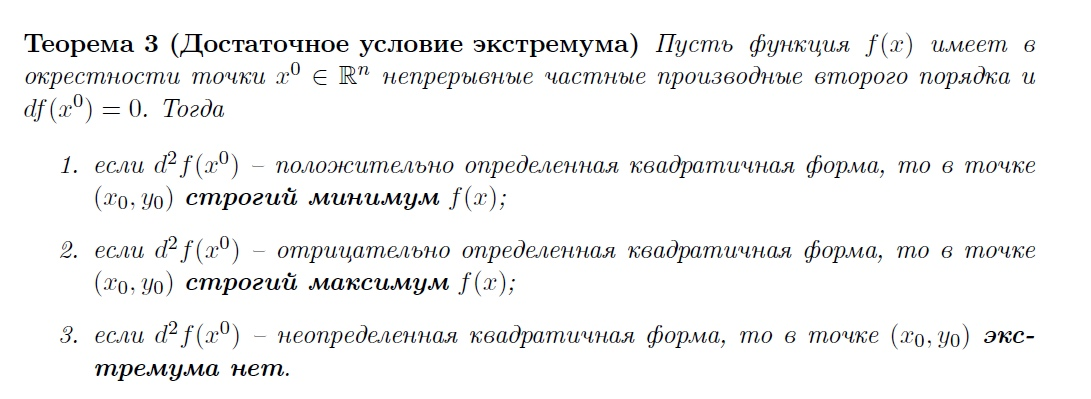
\includegraphics[scale=0.4]{task_2.jpg}}
\end{center}
\newpage
Составим уравнение сферы по известным нам точкам ($R$ -- радиус сферы).

$$ \begin{cases} (0-a)^2+(0-b)^2+(12-c)^2=R^2 \\
                (0-a)^2+(0-b)^2+(4-c)^2=R^2 \\
                (8-a)^2+(0-b)^2+(8-c)^2=R^2
    \end{cases} \,\Rightarrow\,
    \begin{cases} a^2+b^2+(12-c)^2=R^2 \\
                    a^2+b^2+(4-c)^2=R^2 \\
                    (8-a)^2+b^2+(8-c)^2=R^2
    \end{cases}$$

$$ \begin{cases} 128-16c=0 \\
                -16a=8c-112 \\
                b^2=R^2-a^2-c^2-16+8c
    \end{cases} \,\Rightarrow\,
    \begin{cases} a=3 \\
                b=\sqrt{R^2-25} \\
                c=8
    \end{cases}$$
    
Составим уранвение по искомой точке $D(x,y,z)$.
$$ (x-a)^2+(y-b)^2+(z-c)^2=R^2 $$
$$ (x-3)^2+(y-\sqrt{R^2-25})^2+(z-8)^2=R^2 $$
Так как $D\in Oxy$, то $z=0$.
$$ R=\sqrt{(x-3)^2+(y-\sqrt{R^2-25})+64}=\sqrt{x^2-6x+y^2-2y\sqrt{R^2-25}+R^2+48} $$
$$ \begin{cases} R_x'=0 \\
                R_y'=0
    \end{cases} \,\Rightarrow\,
    \begin{cases} \cfrac{x-3}{R}=0 \\
                \cfrac{y-\sqrt{R^2-25}}{R}=0
    \end{cases} \,\Rightarrow\,
    \begin{cases} x=3 \\
                y=\sqrt{R^2-25}
    \end{cases}$$
Критическая точка $M(x,y)=M(3,\sqrt{R^2-25})$. Рассмотрим вторые частные производные в этой точке.
$$ R_{xx}''(M)=\cfrac{R-\frac{x-3}{R}(x-3)}{R^2}=\cfrac{(y-\sqrt{R^2-25})^2+64}{R^3}=8 $$
$$ R_{xy}''(M)=\cfrac{0-\frac{y-\sqrt{R^2-25}}{R}(x-3)}{R^2}=0 $$
$$ R_{yy}''(M)=\cfrac{R-\frac{y-\sqrt{R^2-25}}{R}(y-\sqrt{R^2-25})}{R^2}=\cfrac{(x-3)^2+64}{R^3}=8 $$
Тогда найдем $d^2R$  и исследуем его в точке $M$.
$$ d^2R(M)=R_{xx}''R_{yy}''-R_{xy}''R_{yx}''=64>0 $$
\newpage
Также, $A>0$. Следовательно, по теореме 3 о достаточном условии экстремума, точка $M$ -- точка минимума. Тогда $R_{min}=8$.
Координаты точки $D$ тогда:
$$ x=3,\quad y=\sqrt{R^2-25}=\sqrt{39},\quad z=0 $$
Ответ: точка $D(3,\sqrt{39},0)$.

\paragraph{График (\href{https://www.geogebra.org/3d/fqvczfu9}{нажми на меня})}
\begin{center}
    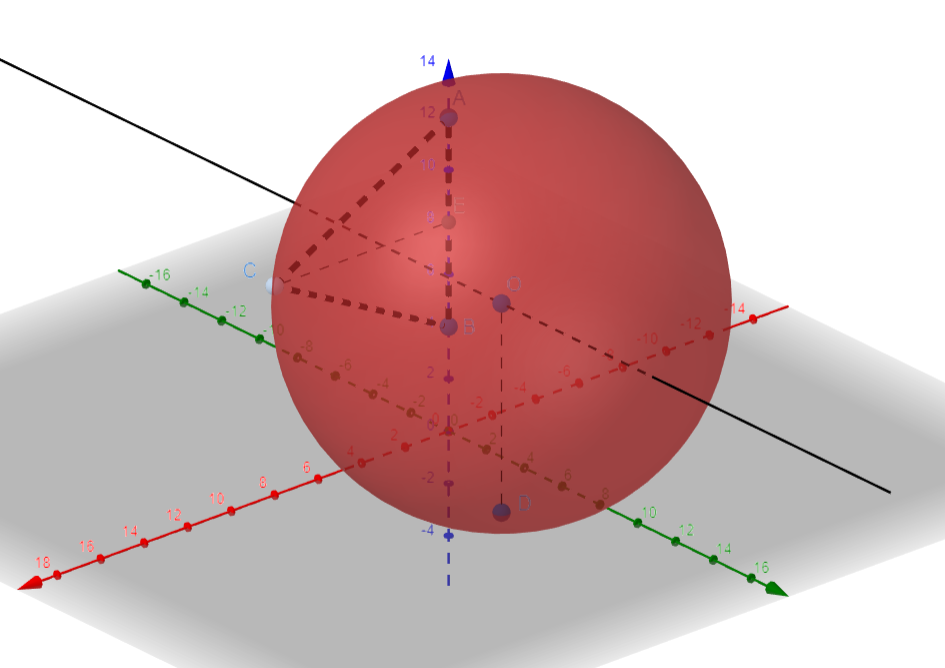
\includegraphics[scale=0.8]{task2.png}
\end{center}
\chapter{Решение дифференциального уравнения в частных
производных с помощью замены переменной}
Решить уравнение, приняв за новые независимые переменные $u$ и $v$, а $w$ -- за
новую функцию:
$$ \frac{\partial z}{\partial y}\Bigg(1+\frac{\partial z}{\partial y}\Bigg)\frac{\partial^2 z}{\partial x^2} - \Bigg(1+\frac{\partial z}{\partial x}+\frac{\partial z}{\partial y}+2\frac{\partial z}{\partial x}\frac{\partial z}{\partial y}\Bigg)\frac{\partial^2 z}{\partial x \partial y}+\frac{\partial z}{\partial x}\Bigg(1+\frac{\partial z}{\partial x}\Bigg)\frac{\partial^2 z}{\partial y^2}=0,$$
если $u=x+z,$ $v=y+z$, $w=x+y+z$.
\chapter{Производная по направлению}
Найти производную функции 
$$f(x,y,z)=ln(e^x,e^y,e^z)$$ 
в направлении луча, образующего с осями координат углы $\frac{\pi}{3},$ $\frac{\pi}{4}$ соответственно и острый угол с осью $Oz$, в данной точке $M(0,0,0)$.

Угол между осью $Oz$ и лучом составляет $\cfrac{\pi}{3}$. 

Зададим вектор $\overline{l}=\big(\cos\cfrac{\pi}{3},\,\cos\cfrac{\pi}{4},\,\cos\cfrac{\pi}{3}\big)$. Тогда производаня функции по вектору $\overline{l}$ равна:

$$ \cfrac{\partial f}{\partial \overline{l}}(M)=(\text{grad}\,f(M),\,\overline{l})=  \evaluat[\Bigg]{\cfrac{e^x}{e^x+e^y+e^z}}_{(0,0,0)} \cdot\cos\cfrac{\pi}{3}+$$

$$+\evaluat[\Bigg]{\cfrac{e^y}{e^x+e^y+e^z}}_{(0,0,0)} \cdot\cos\cfrac{\pi}{4}+\evaluat[\Bigg]{\cfrac{e^z}{e^x+e^y+e^z}}_{(0,0,0)} \cdot\cos\cfrac{\pi}{3}=\cfrac{2+\sqrt{2}}{6}$$



\chapter{Неявная функция}
Определяет ли уравнение 
$$F(\overline{x},y)=\frac{x_1}{y}+ln\frac{y}{x_2}+1=0$$ 
неявную функцию $y=f(x)$ в точке $M(-2,2,2)$? Будет ли эта функция дифференцируема? Если да, найти её полный дифференциал первого порядка и все частные производные второго порядка в точке $M$.

Воспользуемся следующей теорией:
\begin{center}
\fbox{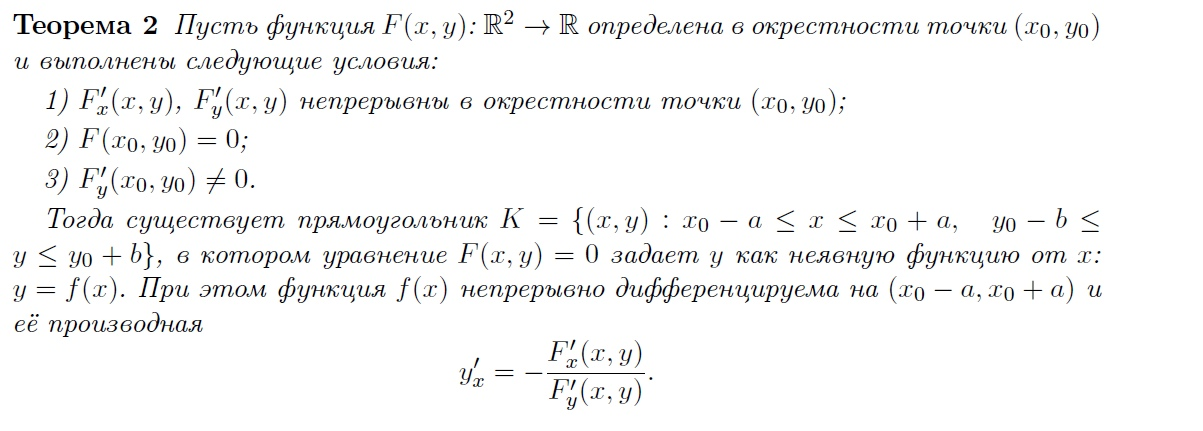
\includegraphics[scale=0.4]{2.jpg}}
\end{center}
\begin{center}
\fbox{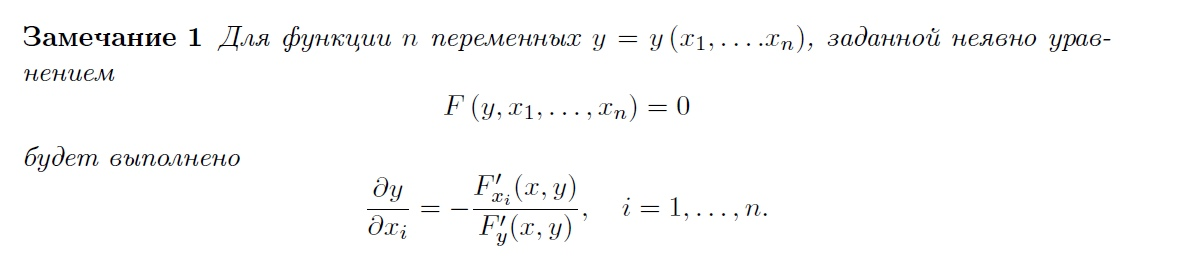
\includegraphics[scale=0.4]{3.jpg}}
\end{center}
Приступим.
\begin{enumerate}
    \item $F_{x_1}'=\cfrac{1}{y}$, $F_{x_2}'=-\cfrac{1}{x_2}$, $F_y' =-\cfrac{x_1}{y^2}+\cfrac{1}{y}$ все непрерывны в окрестности точки $M$.
    \item $F(M)=\cfrac{-2}{2}+ln\cfrac{2}{2}+1=0$
    \item $F_y'(M)=\cfrac{1}{2}+\cfrac{1}{2}\ne0$
\end{enumerate}
Значит, по Теореме 2 уравнение $F(x,y)=0$ задаёт $y=y(x)$ как неявную функцию в окрестности точки $M$, при этом $y(x)$ является непрерывно дифференцируемый в окрестности точки $(x_{1_0}, x_{2_0})$.

Тогда полный дифференциал функции $y(x)$ равен (используя Замечание 1):
$$ \cfrac{\partial y}{\partial x}=\cfrac{\partial y}{\partial x_1}dx_1+\cfrac{\partial y}{\partial x_2}dx_2= -\cfrac{F_{x_1}'(x,y)}{F_y'(x,y)}dx_1 - \cfrac{F_{x_2}'(x,y)}{F_y'(x,y)}dx_2 =\cfrac{y}{x_1-y}dx_1+\cfrac{y^2}{x_2(y-x_1)}dx_2 $$

Частные вторые производные:

$$ \cfrac{\partial^2y}{\partial x_1^2}=\cfrac{\partial}{\partial x_1}\Bigg(\cfrac{\partial y}{\partial x_1}\Bigg)= \cfrac{\cfrac{\partial y}{\partial x_1}(x_1-y)-\Bigg(1-\cfrac{\partial y}{\partial x_1}\Bigg)y}{(x_1-y)^2}=\cfrac{\cfrac{\partial y}{\partial x_1}x_1-y}{(x_1-y)^2}=\cfrac{y^2}{(x_1-y)^3}$$

$$\cfrac{\partial^2y}{\partial x_2\partial x_1}=\cfrac{\partial}{\partial x_2}\Bigg(\cfrac{\partial y}{\partial x_1}\Bigg)=\cfrac{\cfrac{\partial y}{\partial x_2}(x_1-y)+y\cdot\cfrac{\partial y}{\partial x_2}}{(x_1-y)^2}= \cfrac{y^2x_1}{x_2(y-x_1)^3}$$

$$\cfrac{\partial^2y}{\partial x_1\partial x_2}=\cfrac{\partial}{\partial x_1}\Bigg(\cfrac{\partial y}{\partial x_2}\Bigg)= \cfrac{1}{x_2}\cdot\cfrac{2y\cdot\cfrac{\partial y}{\partial x_1}(y-x_1)-y^2\Bigg(\cfrac{\partial y}{\partial x_1}-1\Bigg)}{(y-x_1)^2}=\cfrac{x_1y}{(y-x_1)^3} $$

$$\cfrac{\partial^2y}{\partial x_2^2}=\cfrac{\partial}{\partial x_2}\Bigg(\cfrac{\partial y}{\partial x_2}\Bigg)= \cfrac{2y\cdot\cfrac{\partial y}{\partial x_2}\cdot x_2(y-x_1)-y^2\Bigg(y-x_1+x_2\cdot\cfrac{\partial y}{\partial x_2}\Bigg)}{(x_2(y-x_1))^2}=\cfrac{-y^2x_1^2}{x_2^2(y-x_1)^3} $$

\chapter{Условный экстремум}
С помощью метода Лагранжа исследовать функцию 
$$ f(x,y,z)=x-y+2z $$
на условный экстремум при данном уравнении связи $x^2+y^2+2z^2=16$.
Составим функцию Лагранжа.
$$ L=f(x,y,z)+\lambda \phi(x,y,z)=x-y+2z+\lambda(x^2+y^2+2z^2-16) $$
Частные производные по $x$, $y$, $z$ и $\lambda$.
$$\begin{cases} L_x'=1+2\lambda x=0 \\ L_y'=-1+2\lambda y=0 \\ L_z'=2+4\lambda z=0 \\ x^2+y^2+2z^2-16=0\end{cases} \Rightarrow\quad \begin{cases} x=-\cfrac{1}{2\lambda} \\ y=\cfrac{1}{2\lambda} \\ z=-\cfrac{1}{2\lambda} \\ \lambda=\pm \cfrac{1}{4} \end{cases}$$
Мы получили два значения $\lambda$ (множителя Лагранжа), значит у нас две стационарных точек, подозреваемых в экстремуме. Тогда первая стационарная точка $A=(-2,2,-2)$, а вторая $B=(2,-2,2)$.

Составим квадратичную форму по формуле $d^2L=L_{xx}''dx^2+L_{yy}''dy^2+L_{zz}''dz^2+2L_{xy}''dxdy+2L_{xz}''dxdz+2L_{yz}''dydz $:
$$ d^2L=2\lambda dx^2+2\lambda dy^2 + 2\lambda dz^2=2\lambda(dx^2+dy^2+dz^2) $$
По определению: если $d^2L(Tochka)>0$, то $Tochka$ является точкой строгого условного минимума функции, если $<0$ -- то точкой строгого условного максимума.

$d^2L(A)=\cfrac{1}{2}(dx^2+dy^2+dz^2)>0\,\Rightarrow$ $A$ -- точка условного минимума.

$d^2L(B)=-\cfrac{1}{2}(dx^2+dy^2+dz^2)<0\,\Rightarrow$ $B$ -- точка условного максимума.

\end{document}